\documentclass[journal,12pt,twocolumn]{IEEEtran}
%
\usepackage{setspace}
\usepackage{gensymb}
%\doublespacing
\singlespacing

%\usepackage{graphicx}
%\usepackage{amssymb}
%\usepackage{relsize}
\usepackage[cmex10]{amsmath}
%\usepackage{amsthm}
%\interdisplaylinepenalty=2500
%\savesymbol{iint}
%\usepackage{txfonts}
%\restoresymbol{TXF}{iint}
%\usepackage{wasysym}
\usepackage{amsthm}
%\usepackage{iithtlc}
\usepackage{mathrsfs}
\usepackage{txfonts}
\usepackage{stfloats}
\usepackage{bm}
\usepackage{cite}
\usepackage{cases}
\usepackage{subfig}
%\usepackage{xtab}
\usepackage{longtable}
\usepackage{multirow}
%\usepackage{algorithm}
%\usepackage{algpseudocode}
\usepackage{enumitem}
\usepackage{mathtools}
\usepackage{steinmetz}
\usepackage{tikz}
\usepackage{circuitikz}
\usepackage{verbatim}
\usepackage{tfrupee}
\usepackage[breaklinks=true]{hyperref}
%\usepackage{stmaryrd}
\usepackage{tkz-euclide} % loads  TikZ and tkz-base
%\usetkzobj{all}
\usetikzlibrary{calc,math}
\usepackage{listings}
    \usepackage{color}                                            %%
    \usepackage{array}                                            %%
    \usepackage{longtable}                                        %%
    \usepackage{calc}                                             %%
    \usepackage{multirow}                                         %%
    \usepackage{hhline}                                           %%
    \usepackage{ifthen}                                           %%
  %optionally (for landscape tables embedded in another document): %%
    \usepackage{lscape}     
\usepackage{multicol}
\usepackage{chngcntr}
%\usepackage{enumerate}

%\usepackage{wasysym}
%\newcounter{MYtempeqncnt}
\DeclareMathOperator*{\Res}{Res}
%\renewcommand{\baselinestretch}{2}
\renewcommand\thesection{\arabic{section}}
\renewcommand\thesubsection{\thesection.\arabic{subsection}}
\renewcommand\thesubsubsection{\thesubsection.\arabic{subsubsection}}

\renewcommand\thesectiondis{\arabic{section}}
\renewcommand\thesubsectiondis{\thesectiondis.\arabic{subsection}}
\renewcommand\thesubsubsectiondis{\thesubsectiondis.\arabic{subsubsection}}

% correct bad hyphenation here
\hyphenation{op-tical net-works semi-conduc-tor}
\def\inputGnumericTable{}                                 %%

\lstset{
%language=C,
frame=single, 
breaklines=true,
columns=fullflexible
}
%\lstset{
%language=tex,
%frame=single, 
%breaklines=true
%}

\begin{document}
%


\newtheorem{theorem}{Theorem}[section]
\newtheorem{problem}{Problem}
\newtheorem{proposition}{Proposition}[section]
\newtheorem{lemma}{Lemma}[section]
\newtheorem{corollary}[theorem]{Corollary}
\newtheorem{example}{Example}[section]
\newtheorem{definition}[problem]{Definition}
%\newtheorem{thm}{Theorem}[section] 
%\newtheorem{defn}[thm]{Definition}
%\newtheorem{algorithm}{Algorithm}[section]
%\newtheorem{cor}{Corollary}
\newcommand{\BEQA}{\begin{eqnarray}}
\newcommand{\EEQA}{\end{eqnarray}}
\newcommand{\define}{\stackrel{\triangle}{=}}

\bibliographystyle{IEEEtran}
%\bibliographystyle{ieeetr}


\providecommand{\mbf}{\mathbf}
\providecommand{\pr}[1]{\ensuremath{\Pr\left(#1\right)}}
\providecommand{\qfunc}[1]{\ensuremath{Q\left(#1\right)}}
\providecommand{\sbrak}[1]{\ensuremath{{}\left[#1\right]}}
\providecommand{\lsbrak}[1]{\ensuremath{{}\left[#1\right.}}
\providecommand{\rsbrak}[1]{\ensuremath{{}\left.#1\right]}}
\providecommand{\brak}[1]{\ensuremath{\left(#1\right)}}
\providecommand{\lbrak}[1]{\ensuremath{\left(#1\right.}}
\providecommand{\rbrak}[1]{\ensuremath{\left.#1\right)}}
\providecommand{\cbrak}[1]{\ensuremath{\left\{#1\right\}}}
\providecommand{\lcbrak}[1]{\ensuremath{\left\{#1\right.}}
\providecommand{\rcbrak}[1]{\ensuremath{\left.#1\right\}}}
\theoremstyle{remark}
\newtheorem{rem}{Remark}
\newcommand{\sgn}{\mathop{\mathrm{sgn}}}
\providecommand{\abs}[1]{\left\vert#1\right\vert}
\providecommand{\res}[1]{\Res\displaylimits_{#1}} 
\providecommand{\norm}[1]{\left\lVert#1\right\rVert}
%\providecommand{\norm}[1]{\lVert#1\rVert}
\providecommand{\mtx}[1]{\mathbf{#1}}
\providecommand{\mean}[1]{E\left[ #1 \right]}
\providecommand{\fourier}{\overset{\mathcal{F}}{ \rightleftharpoons}}
%\providecommand{\hilbert}{\overset{\mathcal{H}}{ \rightleftharpoons}}
\providecommand{\system}{\overset{\mathcal{H}}{ \longleftrightarrow}}
	%\newcommand{\solution}[2]{\textbf{Solution:}{#1}}
\newcommand{\solution}{\noindent \textbf{Solution: }}
\newcommand{\cosec}{\,\text{cosec}\,}
\providecommand{\dec}[2]{\ensuremath{\overset{#1}{\underset{#2}{\gtrless}}}}
\newcommand{\myvec}[1]{\ensuremath{\begin{pmatrix}#1\end{pmatrix}}}
\newcommand{\mydet}[1]{\ensuremath{\begin{vmatrix}#1\end{vmatrix}}}
%\numberwithin{equation}{section}
\numberwithin{equation}{subsection}
%\numberwithin{problem}{section}
%\numberwithin{definition}{section}
\makeatletter
\@addtoreset{figure}{problem}
\makeatother

\let\StandardTheFigure\thefigure
\let\vec\mathbf
%\renewcommand{\thefigure}{\theproblem.\arabic{figure}}
\renewcommand{\thefigure}{\theproblem}
%\setlist[enumerate,1]{before=\renewcommand\theequation{\theenumi.\arabic{equation}}
%\counterwithin{equation}{enumi}


%\renewcommand{\theequation}{\arabic{subsection}.\arabic{equation}}

\def\putbox#1#2#3{\makebox[0in][l]{\makebox[#1][l]{}\raisebox{\baselineskip}[0in][0in]{\raisebox{#2}[0in][0in]{#3}}}}
     \def\rightbox#1{\makebox[0in][r]{#1}}
     \def\centbox#1{\makebox[0in]{#1}}
     \def\topbox#1{\raisebox{-\baselineskip}[0in][0in]{#1}}
     \def\midbox#1{\raisebox{-0.5\baselineskip}[0in][0in]{#1}}

\vspace{3cm}


\title{Challenge Problem 2}
\author{Jayati Dutta}





% make the title area
\maketitle

\newpage

%\tableofcontents

\bigskip

\renewcommand{\thefigure}{\theenumi}
\renewcommand{\thetable}{\theenumi}
%\renewcommand{\theequation}{\theenumi}


%\begin{abstract}
%This is a simple document explaining how to determine the QR decomposition of a 2x2 matrix.
%\end{abstract}

%Download all python codes 
%
%\begin{lstlisting}
%svn co https://github.com/JayatiD93/trunk/My_solution_design/codes
%\end{lstlisting}

Download all and latex-tikz codes from 
%
\begin{lstlisting}
svn co https://github.com/gadepall/school/trunk/ncert/geometry/figs
\end{lstlisting}
%


\section{Problem}
The center of the conic section:
\begin{align}
y^2 - 2\sqrt{3}xy + 3x^2 +6x -4y +5 =0
\end{align}

\section{Explanation}

\begin{align}
\vec{V} = \myvec{3 & -\sqrt{3}\\-\sqrt{3} & 1}
\end{align}
and 
\begin{align}
\vec{u} = \myvec{3 \\ -2}\\
f=5
\end{align}
Now, from the eigen values of $\lambda$ =0, 4 we got the eigen vectors. For $\lambda_1$=0, the eigen vector of $\vec{V}$ is $\vec{p_1}$ and for $\lambda_2$=4, the eigen vector of $\vec{V}$ is $\vec{p_2}$ and those are:
\begin{align}
\vec{p_1} = \myvec{1 \\ \sqrt{3}}
\end{align}
and 
\begin{align}
\vec{p_2} = \myvec{-\sqrt{3} \\ 1}
\end{align}
Now,
$\vec{P}$ should be chosen in such a way that $\vec{P}^T = \vec{P}^{-1}$ and 
$\vec{P}^T V \vec{P}$ = $\vec{D}$. but here it is not satisfying these quations. Here, $\vec{P}^{-1} =\frac{1}{4} \vec{P}^T$. Now, in this case we also observed that, 
\begin{align}
4(\vec{V}\vec{c}+\vec{u}) =\eta \vec{p_1}
\end{align}
But this can be written as:
\begin{align}
\vec{V}\vec{c}+\vec{u} =\frac{\eta}{2} \brak{\frac{1}{2}\vec{p_1}}
\end{align}
So, $\vec{P}$ should be selected as :
\begin{align}
\vec{P} = \myvec{\frac{1}{2} & -\frac{\sqrt{3}}{2}\\\frac{\sqrt{3}}{2} & \frac{1}{2}}
\end{align}
If I did it so, then $\mydet{\vec{P}}$=1 and $\vec{P}^{-1}$=$\vec{P}^T$ and $\vec{P}^T \vec{V} \vec{P}$=$\vec{D}$.
So,
\begin{align}
\vec{p_1} = \myvec{\frac{1}{2} \\ \frac{\sqrt{3}}{2}}
\end{align}
and 
\begin{align}
\vec{p_2} = \myvec{-\frac{\sqrt{3}}{2}\\\frac{1}{2}}
\end{align}
Now, $\eta$ can be calculated as : 
\begin{align}
\eta = 2 \vec{p_1}^T \vec{u}\\
\eta = 2 \myvec{\frac{1}{2} & \frac{\sqrt{3}}{2}} \myvec{3 \\ -2}\\
\eta =  3-2\sqrt{3}
\end{align}
Now, 
\begin{align}
\vec{u}^T + \frac{\eta}{2}\vec{p_1}^T = \myvec{\frac{15-2\sqrt{3}}{4} & \frac{-14+3\sqrt{3}}{4}}\\
\frac{\eta}{2} \vec{p_1} -\vec{u}= \frac{3-2\sqrt{3}}{2}\myvec{\frac{1}{2}\\ \frac{\sqrt{3}}{2} } - \myvec{3\\-2}\\
\frac{\eta}{2} \vec{p_1} -\vec{u}=\myvec{\frac{-9-2\sqrt{3}}{4}\\\frac{2+3\sqrt{3}}{4}}
\end{align}

Now considering the augmented matrix,
\begin{align}
\myvec{\frac{15-2\sqrt{3}}{4} & \frac{-14+3\sqrt{3}}{4} & -5\\3 & -\sqrt{3} & \frac{-9-2\sqrt{3}}{4}\\-\sqrt{3} & 1 & \frac{2+3\sqrt{3}}{4}}\xleftrightarrow[]{R_2\leftarrow R_2/\sqrt{3}}\\
\myvec{\frac{15-2\sqrt{3}}{4} & \frac{-14+3\sqrt{3}}{4} & -5\\\sqrt{3} & -1 & \frac{-(2+3\sqrt{3})}{4}\\-\sqrt{3} & 1 & \frac{2+3\sqrt{3}}{4}}\\
\xleftrightarrow[R_2\leftarrow R_2/\sqrt{3}]{R_3\leftarrow R_2+R_3}\\
\myvec{\frac{15-2\sqrt{3}}{4} & \frac{-14+3\sqrt{3}}{4} & -5\\1 & -\frac{1}{\sqrt{3}} & -\frac{-(2+3\sqrt{3})}{4\sqrt{3}}\\0 & 0 & 0}\\
\xleftrightarrow[]{R_1\leftarrow R_1/\frac{15-2\sqrt{3}}{4}}
\myvec{1 & \frac{-14+3\sqrt{3}}{15-2\sqrt{3}} & -\frac{5}{15-2\sqrt{3}}\\1 & -\frac{1}{\sqrt{3}} & -\frac{-(2+3\sqrt{3})}{4\sqrt{3}}\\0 & 0 & 0}\\
\xleftrightarrow[]{R_2\leftarrow R_2-R_1}
\myvec{1 & \frac{-14+3\sqrt{3}}{15-2\sqrt{3}} & -\frac{5}{15-2\sqrt{3}}\\0 & -\frac{24-16\sqrt{3}}{15\sqrt{3}-6} & \frac{-12+39\sqrt{3}}{4\sqrt{3}(15-2\sqrt{3})}\\0 & 0 & 0}
\end{align}
So, 
\begin{align}
\myvec{1 & \frac{-14+3\sqrt{3}}{15-2\sqrt{3}}\\0 & -\frac{24-16\sqrt{3}}{15\sqrt{3}-6}}\vec{c}=\myvec{-\frac{5}{15-2\sqrt{3}}\\\frac{-12+39\sqrt{3}}{4\sqrt{3}(15-2\sqrt{3})}}\\
\implies c_2= -\frac{-12+39\sqrt{3}}{4(24-16\sqrt{3})}\\
\implies c_2 = 3.74\\
c_1=1.12
\end{align}
From there we can get $\vec{c}$=$\myvec{1.12\\3.74}$. The vertex of parabola will be at (1.12, 3.74).

\begin{figure}[!ht]
\centering
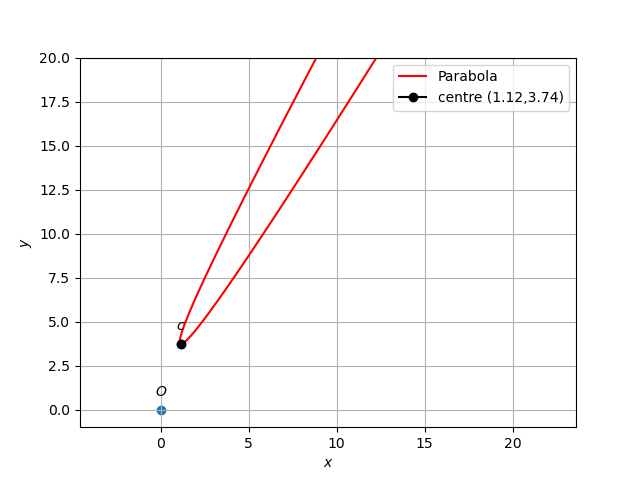
\includegraphics[width=\columnwidth]{./figs/parabola_4.png}
\caption{Parabola}
\label{fig:parabola}
\end{figure}

\renewcommand{\theequation}{\theenumi}
\begin{enumerate}[label=\thesection.\arabic*.,ref=\thesection.\theenumi]
\numberwithin{equation}{enumi}
\item Verification of the above problem using python code.\\
\solution The  following Python code generates Fig. \ref{fig:parabola}
\begin{lstlisting}
codes/check_parab.py
\end{lstlisting}

So the solution is matching with the given plot, hence it is verified.
%
\end{enumerate}

\end{document}



